%
% Project documentation template
% ===========================================================================
% This is part of the document "Project documentation template".
% Authors: brd3, kaa1
%

\begin{titlepage}


% BFH-Logo absolute placed at (28,12) on A4 and picture (16:9 or 15cm x 8.5cm)
% Actually not a realy satisfactory solution but working.
%---------------------------------------------------------------------------
\setlength{\unitlength}{1mm}
\begin{textblock}{20}[0,0](28,12)
	
\includegraphics[scale=1.0]{images/BFH_Logo_B.png}
\end{textblock}

\begin{textblock}{154}(28,48)
	\begin{picture}(150,2)
		\put(0,0){\color{bfhgrey}\rule{150mm}{2mm}}
	\end{picture}
\end{textblock}

\begin{textblock}{154}[0,0](28,50)
	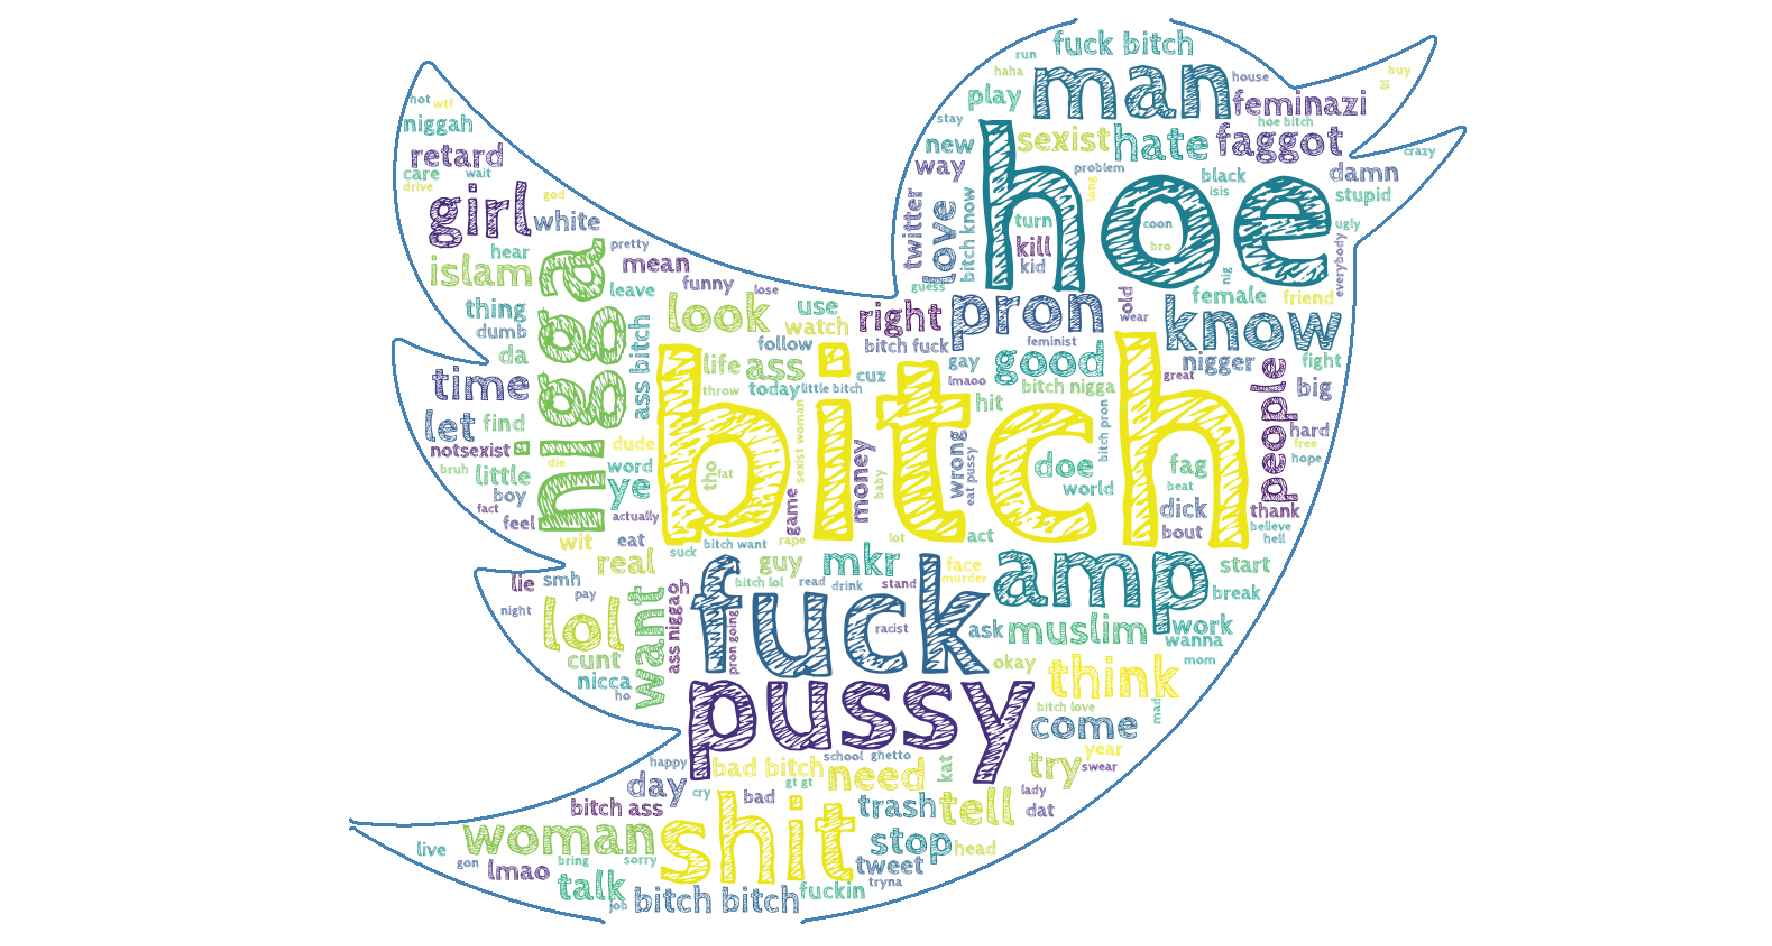
\includegraphics[scale=1.0]{images/abusive_twitter_wordcloud.png}			% define cover picture
\end{textblock}

\begin{textblock}{154}(28,135)
	\begin{picture}(150,2)
		\put(0,0){\color{bfhgrey}\rule{150mm}{2mm}}
	\end{picture}
\end{textblock}
\color{black}

% Institution / titel / subtitel / authors / experts:
%---------------------------------------------------------------------------
\begin{flushleft}

\vspace*{115mm}

\fontsize{26pt}{28pt}\selectfont
\heading				\\							% Read heading from file leader/title.tex
\vspace{2mm}

%\fontsize{16pt}{20pt}\selectfont\vspace{0.3em}
%Detection of hate speech and abusive language in tweets.		\\				% Insert subheading
%\vspace{5mm}

\fontsize{10pt}{12pt}\selectfont
\textbf{Semesterarbeit} \\		% Insert text
\vspace{3mm}

% Abstract (eingeben):
%---------------------------------------------------------------------------
\begin{textblock}{150}(28,190)
\fontsize{10pt}{12pt}\selectfont
Zusammen mit der massiven Zunahme der Nutzung von Social Media ist eine Zunahme von hasserf{\"u}llten und missbr{\"a}uchlichen {\"A}usserungen zu beobachten.
Diese Semesterarbeit beschreibt den Aufbau einer Streaming und Analyse Umgebung f{\"u}r Twitter-Feeds, welche einerseits in grossen Mengen zum Training f{\"u}r sp{\"a}tere Machine Learning Algorithmen gesammelt werden und andererseits durch bereits bestehende Algorithmen klassifiziert und in einem Analyse Dashboard visualisiert werden.
\end{textblock}

\begin{textblock}{150}(28,225)
\fontsize{10pt}{17pt}\selectfont
\begin{tabbing}
xxxxxxxxxxxxxxx\=xxxxxxxxxxxxxxxxxxxxxxxxxxxxxxxxxxxxxxxxxxxxxxx \kill
Degree course:	\> CAS Big Data 2019	\\		% insert name of degree course
Author:		\> Verena Mai		\\					% insert names
Experts:		\>  J{\"u}rgen Eckerle				\\							% insert names
Date:			\> \versiondate					\\							% read from file leader/version.tex
\end{tabbing}

\end{textblock}
\end{flushleft}

\begin{textblock}{150}(28,280)
\noindent
\color{bfhgrey}\fontsize{9pt}{10pt}\selectfont
Berner Fachhochschule | Haute \'ecole sp\'ecialis\'ee bernoise | Bern University of Applied Sciences
\color{black}\selectfont
\end{textblock}


\end{titlepage}

%
% ===========================================================================
% EOF
%
